\chapter{Introduction}

\section{Background}
Capacitive touchscreens are one of the most profound interaction interfaces on modern devices. Benefit from the sensitivity and robustness of capacitive touchscreen, it is able to provide seamless, intuitive interaction between users and digital media. Furthermore, comparing with resistive touchscreen, the possibility of multitouch enabled by capacitive touchscreen as well as the unbreakable freature makes it a dominance in the touchscreen market. However, capacitive screen is still relatively expensive comparing with resistive touchscreen. Though manufactures launched various different large-scale capacitive-screen products such as touchscreen wall, touchscreen table, touchscreen board, etc ~\ref{fig:touchscreen-products}, the price of these products are unaffordable to ordinary people, due to the cost of capacitive touchscreen per unit area. As the most affordable touchscreen products, smartphone's touch interface is still limited to the area where touch sensors are embedded, constraining natural user interactions to the surfaces of these smart devices. Therefore, simply scaling touchscreens to large surfaces and everyday objects is expensive and challenging, which limits its wider adoption in the Internet of Things applications. How to scale the sensing capability of small capacitive touchscreen to larger area in a low-cost manner to enable large-scale touch interactions has become a popular research topic in the field of Human Computer Interaction.

% \begin{figure}[ht]
%   \centering
%     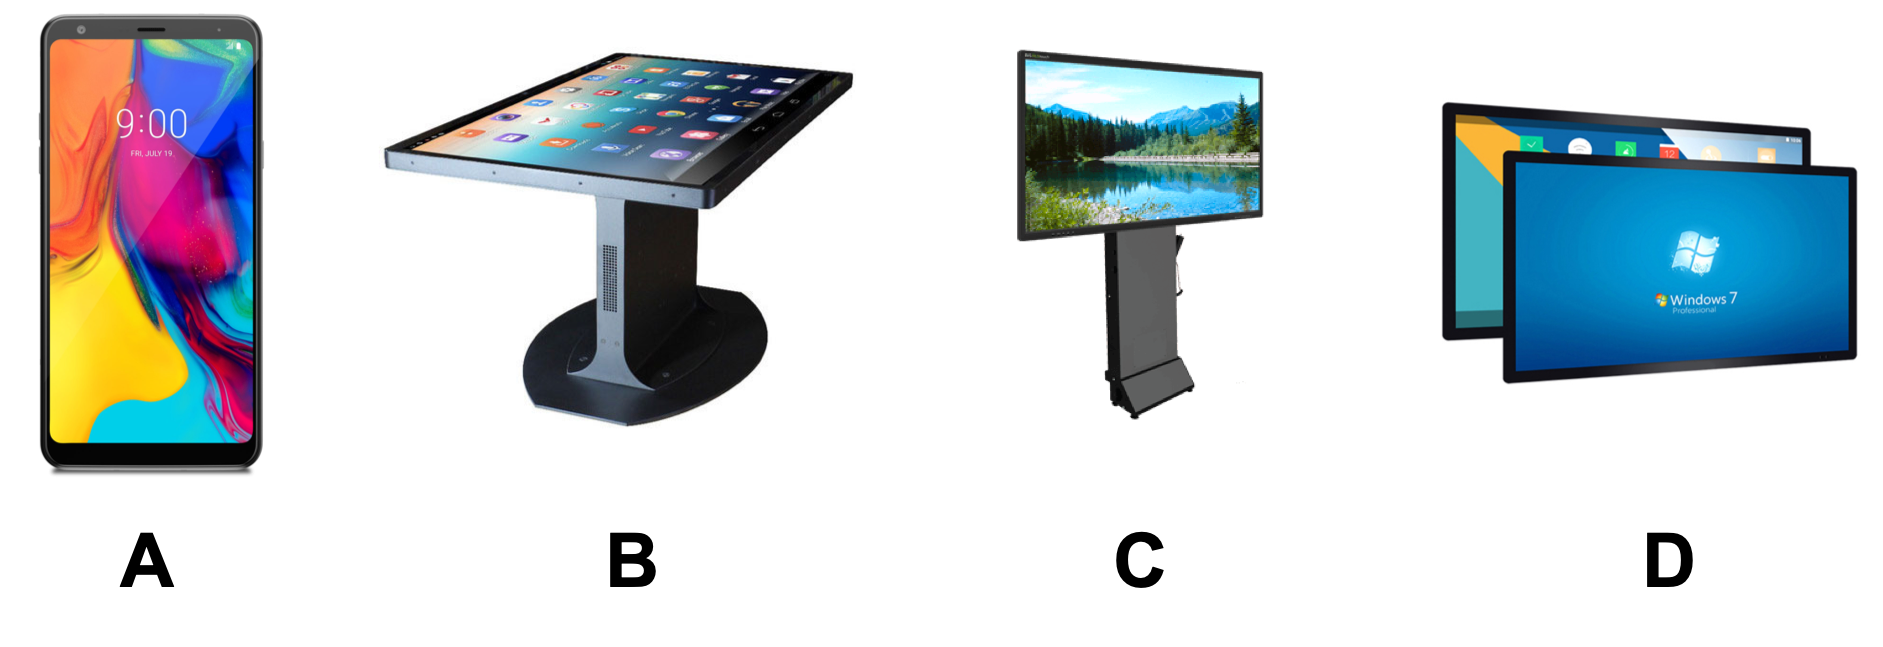
\includegraphics[width=0.8\columnwidth]{figures/touchproducts.png}
%     \setlength{\belowcaptionskip}{-8pt}
%     \caption{Capacitive touchscreen products: iphone (A). multitouch arcade touchscreen game table (B) interactive whiteboard (C). touchscreen Wall (D).}
%     \label{fig:touchscreen-products}
  
% \end{figure}

Researchers have explored enabling touch interfaces on everyday surfaces or objects ~\cite{Ono-Touch-and-Activate, Ono-2014,Sato-Touche, Xiao-WorldKit, Rekimoto-SmartSkin, olberding2013cuttable, Zhang-Electrick} with various sensing techniques. However, to recognize the touch events on everyday objects such as toys, it requires different embedded sensors, such as resonate sensor, capacitive touch sensor, volatage sensor, and camera. 

As we can see, these prior works require dedicated sensing platforms such as Arduino to power touch interfaces and to enable wireless communication with digital devices. These requirements prevent end-users from easily fabricating customizable touch interfaces. Users need to dedicately coporate the sensors with the touch interface and need to build companion computer program for event recognition, which significantly raise the barrier for fast prototyping. 

As an alternative, in recent 5 years, researchers are trying to leverage the existing sensors that are available to everyone to empower everyday objects with sensing capability. Thanks to the ubiquity of capacitive touchscreen device such as smartphone, ipad and latop, researchers have proposed extending the capacitive sensing capability of these touchscreen devices to ambient surfaces through conductive strips. These systems can support interactions such as touch widgets ~\cite{Kato2015a,Kato2015,Kato2016}, trackpad ~\cite{mobicom-gao18} as well as tangible interfaces ~\cite{Schmitz2017, Schmitz2018, Chan-CapStones}. However, though these systems is able to provide interaction beyond touchscreen surface, due to the lack of raw capacitance siganl, the smart device fail to distinguish the touch event between on-screen touch and off-screen touch, which will influence user's normal interaction on touchscreen such as click and slide. Additionaly, these approaches can only support applications with very limited sensing range and fabrication materials. Furthermore, the feasibility of long-range capacitive sensing, the design scope, as well as the applications and user case haven't been fully explored.

Our work focuses on two parts: First, we study the feasibility of augmenting the interaction patterns of existing touchscreen device, such as backboard interaction, edge interaction, without disturbing user's on-screen interactions. We demonstrated that by capturing and analyzing the raw capaitance data of touchscreen device such as smartphone, we can configure a special capacitance threshold to accurately seperate on-screen touch event from off-screen touch event. Based on that, we proposed a series of applications to augment user's interaction experience with ambient surfaces of touchscreen devices (Fig ~\ref{fig:small-scale-scenarios}). Second, we dive deeper into the study of large-scale capacitive sensing using existing capacitivve touchscreen devices and conductive materials. Our study shows the possibility of large-scale capacitive sensing. We measured the sensing space of smartphone and proposed two major design patterns of touch interface. Furthermore, we presented example interactive applications of our large-scale sensing technique (Fig ~\ref{fig:large-scale-scenarios}), which is a good alternative of existing large-scale interaction devices such as touch table and touchboard.

% \begin{figure}
  % small scale interaction scenarios
% \end{figure}

% \begin{figure}
% \centering
%   \includegraphics[width=0.78\columnwidth]{figures/scenarios-ubicomp.png}
%   \setlength{\belowcaptionskip}{-8pt}
%   \caption{\textit{FlexTouch} supports various large-scale applications with different configurations. A: Discrete and 1-dimension touch widgets sensing long-range touch events. B: Fitness tracking using designs in A for the count of repetitions, distance and speed measurement on a treadmill, cycling and chest exercise machine. C: Body posture detection on the yoga mat with a built-in capacitive sensing matrix in an X-Y layout. D: Smart desk application for object presence and user's state detection. E. Smart mattress for sleep monitoring with a one-on-one mapping node matrix from the touchscreen.}
%   \label{fig:large-scale-scenarios}
% \end{figure}

\section{Thesis Structure}
In this paper, we present \textit{FlexTouch}, a technique for distinguishing off-screen touch from on-screen touch as well as enabling long-range touch sensing interfaces beyond commercial touchscreens by leveraging a variety of flexible conductive materials (Fig ~\ref{fig:small-scale}, Fig ~\ref{fig:large-scalescenarios}). \textit{FlexTouch} utilizes simple fabrication techniques to create a variety of passive, conductive 2D-patterned touch interfaces that enable new health and wellness applications. 

In chapter 2, we will introduce related works that is relevant to \textit{FlexTouch}. First, we gathered the current literature aiming at enabling touch interaction on everyday surfaces and objects, including both small-scale and large-scale. We will introduce some techniques these papers applied such as capacitive sensing, volatage sensing, camera sensing, etc. Then we review works specifically relevant to capacitive sensing beyond touchscreen surfaces. Finally, we discuss the limitation of prior works regarding capacitive sensing and room for innovation and improvement.

Chapter 3 lays out the theoretical principal of 2D capacitive sensing. We present equivalent circuit to explain the effect of attaching conductive materials on touchscreen as well as the effect of off-screen finger touch. Then we elaborate the reason why large-scale capacitive sensing is so difficult and why introducing local ground will amplify the capacitance siganl. Based on the equivalent circuit, we give a reasonable assumption that the mutual capacitance scales with the area of extended conductive materials.

Chapter 4 first introduces the signal processing algorithm and procedures of recognizing touch event. Then, we propose several different conductive materials as well as fabrication methods for \textit{FlexTouch} implementation. In particularly, we design a clip-on widget, which we called \textbf{plug and play} interface,  that is able to connect the touchscreen to large interactive surface using copper foil tape.

Chapter 5 conducts a series of evalutaion of \textit{FlexTouch}. The first experiment we conduct is observing the difference of signal pattern between on-screen and off-screen touch. Then we explore the relationship between sensing range and coverage area with different conductive materials, hardward and local ground. To step further into studying the effect of grounding strip, which includes the gap between grounding and signal strip, the width of grounding strip, and the conductivity of grounding strip. Finally, to explore the possibility of detecting the presence of everyday objects, we also evaluated the signal variance of touch event across different objects.

In chapter 6, we focus on real-word applications of \textit{FlexTouch}. The applications of \textit{FlexTouch} can be categorized into two different divisions. The first is what we called \textbf{touchscreen ambient interaction}, second is \textbf{larage-scale extendable interaction}. In the first set of applications, we propose four different scenarios, that are direct augmentation of existing touch interactions around smartphones, such as hold-gesture sensing, backboard touch sensing, external plugin flexible keyboard and VR cardboard interaction. In the second part, we present also four common use cases including smart mattress, yoga mat fitness posture detection, fitness tracking, and smart desk. Additionally, we also conduct concrete user study and quantitative analysis on each application to guarantee the feasibility and robustness of \textit{FlexTouch}.  

As a summary of this paper, chapter 7 concludes our work on extending sensing capability of touchscreen surfaces and potential applications. Fianlly, it points out the future direction of our work from three perspectives.

\section{Main Contributions}
Our contributions in this paper are as follow:

1. We differentiated the off-screen touch from on-screen touch, which enables recognizing user's off-screen touch event without disturbing normal on-screen touch event. 

2. We created techniques that leverage a variety of conductive materials and fabrication methods to customize extensions of touchscreens to support continuous 2D touch on everyday objects and ambient surfaces.

3. We enabled large-scale touch sensing up to 4 meters and objects' presence up to 2 meters away from the capacitive touchscreen to ambient surroundings by including the local ground in the external conductive pattern design. 

4. We demonstrated that \textit{FlexTouch} is easy to fabricate, assemble and use. The 2D circuit-like pattern is compatible with various conductive materials (copper foil tape, silver nanoparticle ink, ITO frames, and carbon paint), as well as fabrication methods (cutting, coating, and ink-jet printing). Furthermore, we proposed two easy attaching and assembling approaches to connect the extension part to touchscreens. 

5. We benchmarked the performance of \textit{FlexTouch} through user studies. In particularly, we fully explored design variables such as materials, extension strips' width as well as gap distance between strips and evaluated their impact on the coverage distance of \textit{FlexTouch}. 

6. We demonstrated the versatility and feasibility of \textit{FlexTouch} through multiple applications such as body posture sensing, object presence detection, enhanced fitness sensing applications, etc.

